\documentclass[10pt]{beamer}

\usepackage{amssymb,amsthm}% http://ctan.org/pkg/amssymb
\newtheorem{proposition}{Proposition}
\setbeamertemplate{theorems}[numbered]
\usecolortheme[RGB={100,0,0}]{structure}
\setbeamercolor{block title}{use=structure,fg=white,bg=structure.fg!75!black}
\setbeamercolor{block body}{parent=normal text,use=block title,bg=block title.bg!10!bg}

\usepackage{amsmath}
\DeclareMathOperator*{\argmax}{argmax}
\DeclareMathOperator*{\argmin}{argmin}

\usepackage{natbib}
\bibliographystyle{aea}

\usepackage{xcolor}
\usepackage{graphicx}
\usepackage{amsmath}
\usepackage{numprint}
\npdecimalsign{.}
\nprounddigits{3}
\usepackage{colortbl}
\usepackage{appendixnumberbeamer}
\usepackage{subfigure}
\usepackage{comment}

%\usepackage[hyperref]{beamerarticle} or 
\usepackage{hyperref}
\usepackage{caption}
%\captionsetup{font=scriptsize,labelfont=scriptsize}
\setbeamerfont{caption}{size=\scriptsize}
\usetheme{Singapore}
\usecolortheme{beaver}

% for adding regression tables
\usepackage{dcolumn} 
% column to line up decimals
\usepackage{booktabs,caption}
\captionsetup[table]{name=Table} 
\usepackage[flushleft]{threeparttable} 
% The above two allow that last line with the dagger as a bottom note.
\captionsetup{skip=0pt}

\usepackage{xcolor}
\definecolor{underbrace}{RGB}{30,199,166}
\newcommand{\textfrac}[1]{
  \begin{tabular}{@{}l@{}}#1\end{tabular}
}

\begin{document}

\title{Global Monetary Policy Shocks, Financial Friction and Export Prices}
\author[Yao Amber LI, Lingfei LU and Jingbo YAO]{Yao Amber LI, Lingfei LU, Jingbo YAO}
\institute{\small HKUST}
\date{Dec 1, 2023}

\begin{frame}
\maketitle
\centering
HKUST Research Postgraduate Student Workshop
\end{frame}

\begin{frame}
\frametitle{Outline}
\tableofcontents
\end{frame}

%%%%%%%%%%%%%%%%%%%%%%%%%%%%%%%%%%%%%%%%%%%%%%%%%%%%%%
%%%%%%%%%%%%%%%%%%%%%%%%%%%%%%%%%%%%%%%%%%%%%%%%%%%%%%
\section{I. Introduction}

\begin{frame}{Motivation}
\begin{itemize}
    \item How export price responds to global shocks is essential in international economics
    \medskip
    \item Financial friction affects firms' exporting behavior
    \medskip
    \item International monetary shocks are the main driver of the global financial cycle
    \medskip
    \item  In an era of growing global financial and trade integration, understanding how global monetary shocks affect export prices by affecting firms' financial conditions is quite important
    \medskip

\end{itemize}
\end{frame}

\begin{frame}{This paper}
\begin{itemize}
    \item Using high-frequency exogenous monetary shocks, monthly custom transaction records, and comprehensive firm-level balance sheet data
    \medskip
    \item  A tightening US monetary policy shock significantly increases China's export prices through both the borrowing cost and liquidity channels.
    \medskip
    \item This impact is more pronounced for firms facing higher borrowing costs and tighter liquidity conditions. 
    \medskip
    \item A classical trade model that incorporates financial friction and external monetary policy shocks.
\end{itemize}
\end{frame}


\begin{frame}{Literature}

\begin{itemize}
    \item Financial friction and international trade
    \begin{itemize}
        \item Sector-specific and time-invariant constraint: \cite{manova2013credit}, \cite{lin2018international}
        \item This paper: firm-level time-varying constraint and the role of global monetary shocks
    \end{itemize}
    \item Determinants of export prices
        \begin{itemize}
        \item  Exchange rate shocks: \cite{amiti2014importers}, \cite{auer2018quality}.
        \item Other factors like firm characteristics, destinations, and trade liberalization:  \cite{manova2012export}, \cite{fan2015trade}, etc.
        \item This paper: global monetary policy shocks
    \end{itemize}
    \item Global monetary policy spillover
        \begin{itemize}
        \item Real economy: \cite{bluedorn2011open},  and \cite{di2023impact}
        \item Asset prices: \cite{rogers2014evaluating}, \cite{miranda2020us}.
        \item This paper: exporter behaviors
    \end{itemize}
    \medskip

\end{itemize}

\end{frame}

%%%%%%%%%%%%%%%%%%%%%%%%%%%%%%%%%%%%%%%%%%%%%%%%%%%%%%
%%%%%%%%%%%%%%%%%%%%%%%%%%%%%%%%%%%%%%%%%%%%%%%%%%%%%%
\section{II. Data}

\begin{frame}{Data: Monetary Policy Shock}
    \begin{itemize}
        \item First, we use a US monetary policy shock series developed by \cite{bu2021unified}.
        \begin{itemize}
            \item This measure uses \cite{fama1973risk} two-step partial-least squares estimation using FOMC announcements.
        \end{itemize}
        \item This measure has several advantages:
        \begin{enumerate}
            \item It is largely unpredictable from past available information so that we can regard it as exogenous for the US and other countries;
            \item Its information effect is not significant (pure policy shock);
            \item This unified measure is comparable across the conventional and unconventional monetary policy regimes.
        \end{enumerate}
        \item We also use alternative measures for monetary policy shocks from \cite{nakamura2018high}, \cite{guraynak2005actions}, and \cite{jarocinski2020deconstructing}.
    \end{itemize}
\end{frame}

\begin{frame}{Data: Monetary Policy Shock}
    \begin{itemize}
        \item The whole series is from 1994 to 2022. Within the matched sample, we will focus on the period from 2000 to 2006, 84 months.
    \end{itemize}
    \begin{figure}[htbp]
	\centering
	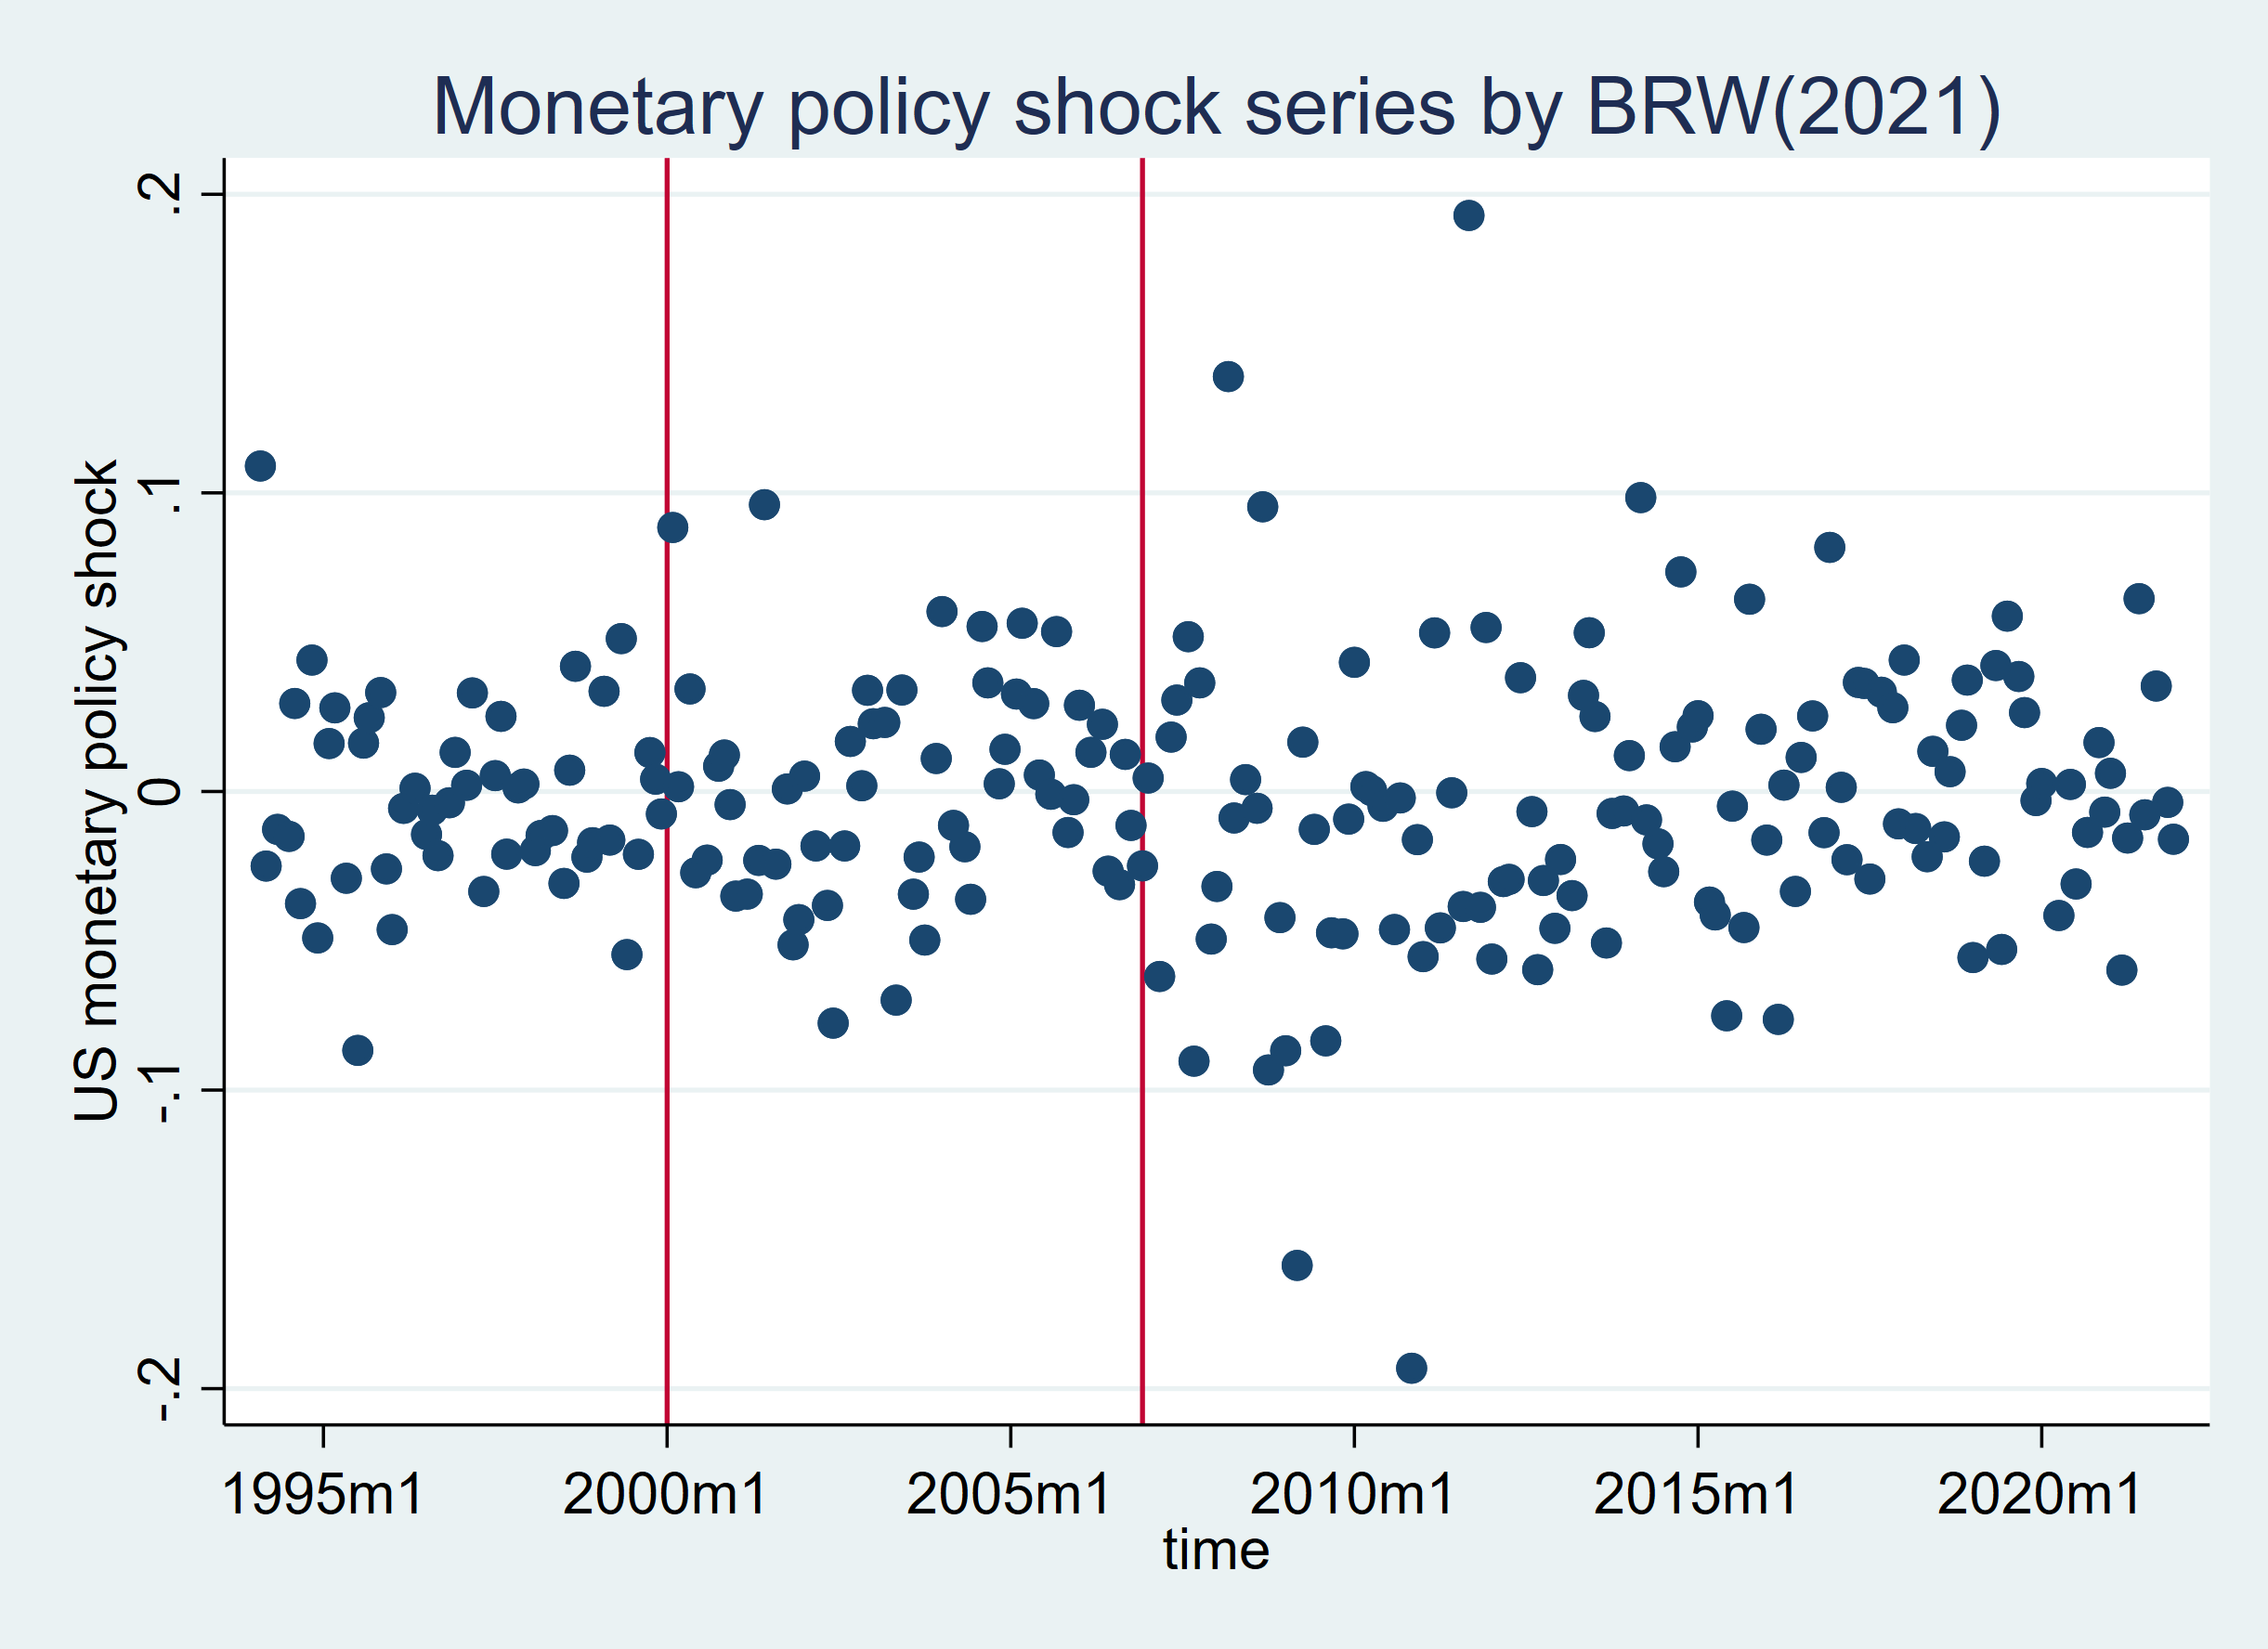
\includegraphics[width=0.8\columnwidth]{latex/drafts/pic/BRW.png}
	\label{sum.brw}
    \end{figure}
\end{frame}

\begin{frame}{Data: Firm-level Information}
	\begin{itemize}
		\item Second, we use annual surveys of Chinese manufacturing firms conducted by the National Bureau of Statistics of China (NBSC).
		\begin{itemize}
			\item This dataset covers all state-owned enterprises and above-scale firms with annual sales of more than 5 million RMB from 1999 to 2007.
			\item The data provide details about firms' identification codes, ownership, industry type, and 80 other balance sheet variables.
                \item To merge firm data with customs records, we match identification codes using firms' contact information (\cite{fan2015trade}).
		\end{itemize}
            \item Our research will focus on the variables related to two aspects:
            \begin{enumerate}
                \item production costs and sales, including total wage payment, total operation inputs, sales income, etc.
                \item financial costs and liquidity conditions, including financial expense and interest payment, total and net working capital, cash holding.
            \end{enumerate}
	\end{itemize}
\end{frame}

\begin{frame}{Data: Customs Transaction Records}
    \begin{itemize}
	\item Finally, we use trade transaction records from the General Administration of Customs of China (GACC).
	\begin{itemize}
		\item This dataset provides universal information on Chinese trade transactions, including import and export values, quantities, product names and codes, source and destination countries, and firm types.
            \item The monthly firm-level transaction records range from 2000-2006.
	\end{itemize}		
    \end{itemize}
    \begin{figure}[htbp]
	\centering
	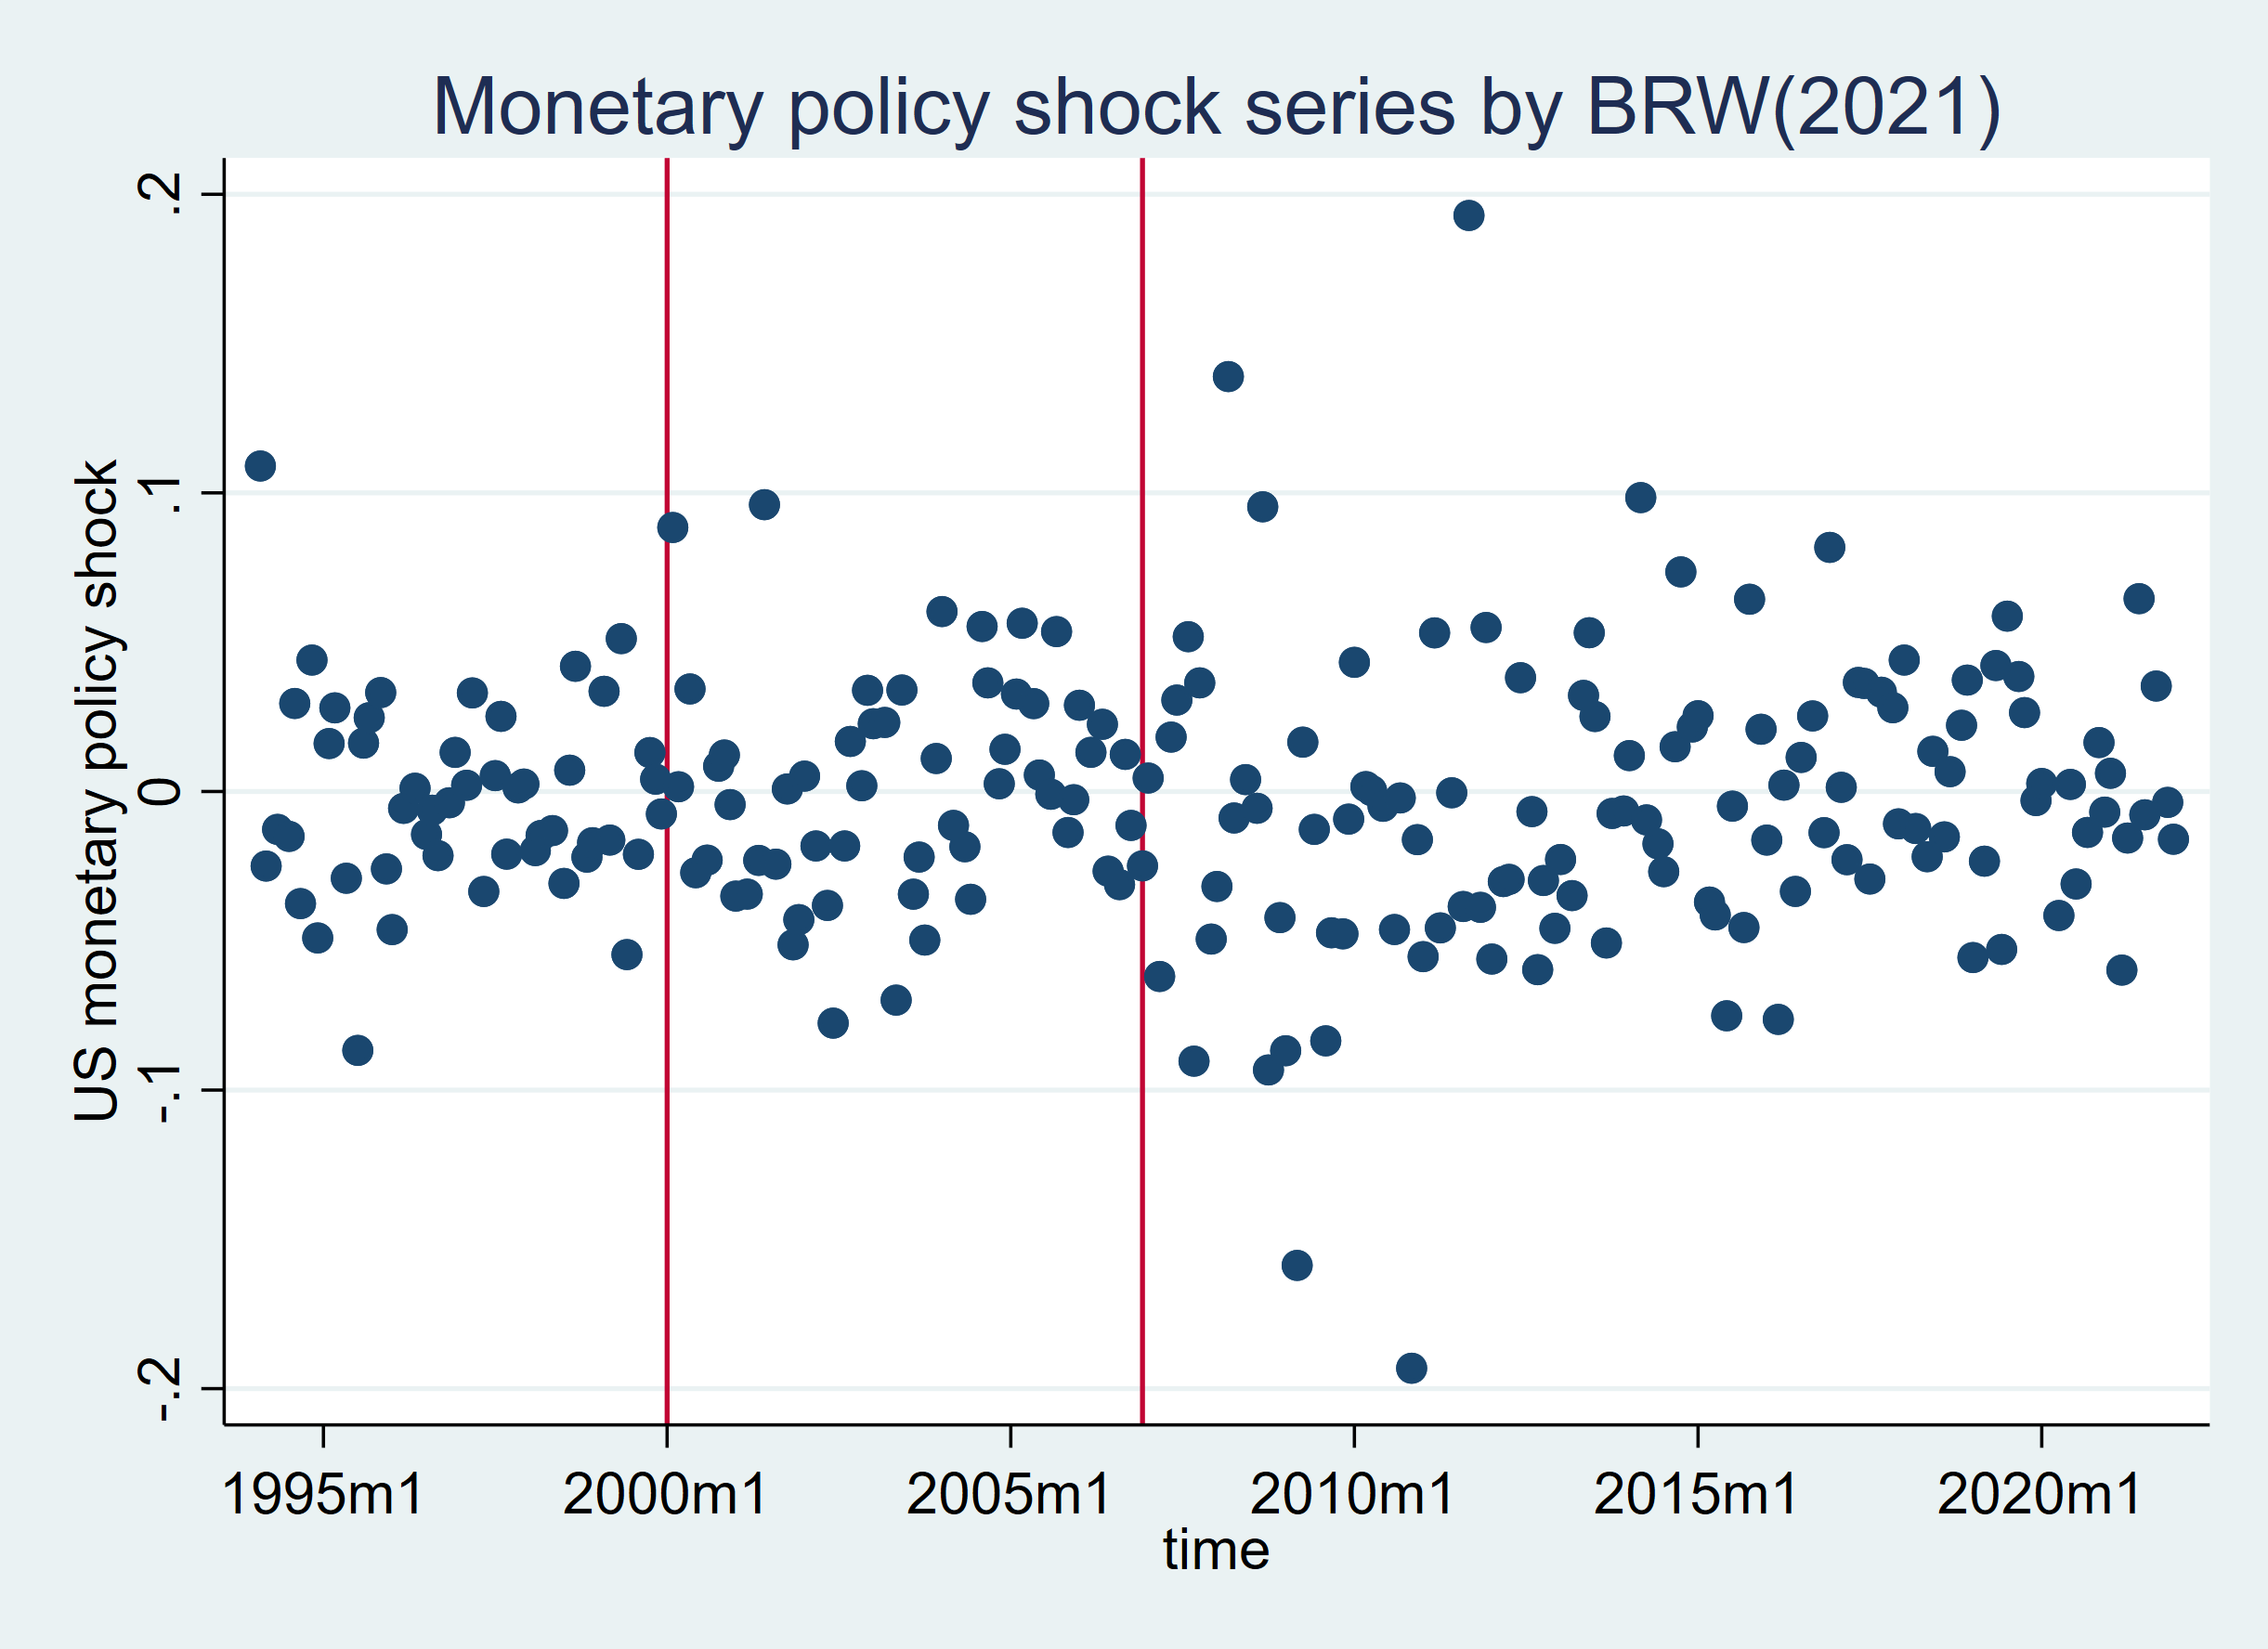
\includegraphics[width=0.8\columnwidth]{latex/drafts/pic/BRW.png}
	\label{sum.brw}
    \end{figure}
\end{frame}

%%%%%%%%%%%%%%%%%%%%%%%%%%%%%%%%%%%%%%%%%%%%%%%%%%%%%%
%%%%%%%%%%%%%%%%%%%%%%%%%%%%%%%%%%%%%%%%%%%%%%%%%%%%%%
\section{III. Empirical Results}

\begin{frame}{}
\begin{itemize}
    \item 
    \medskip

\end{itemize}
\end{frame}

%%%%%%%%%%%%%%%%%%%%%%%%%%%%%%%%%%%%%%%%%%%%%%%%%%%%%%
%%%%%%%%%%%%%%%%%%%%%%%%%%%%%%%%%%%%%%%%%%%%%%%%%%%%%%
\section{IV. Mechanism}
\begin{frame}{}
\begin{itemize}
    \item 
    \medskip

\end{itemize}
\end{frame}

%%%%%%%%%%%%%%%%%%%%%%%%%%%%%%%%%%%%%%%%%%%%%%%%%%%%%%
%%%%%%%%%%%%%%%%%%%%%%%%%%%%%%%%%%%%%%%%%%%%%%%%%%%%%%
\section{V. More Discussion}
\begin{frame}{}
\begin{itemize}
    \item 
    \medskip

\end{itemize}
\end{frame}

%%%%%%%%%%%%%%%%%%%%%%%%%%%%%%%%%%%%%%%%%%%%%%%%%%%%%%
%%%%%%%%%%%%%%%%%%%%%%%%%%%%%%%%%%%%%%%%%%%%%%%%%%%%%%
\section{VI. Model}

\begin{frame}{Preferences and demand}

We here introduce a general trade model like Meliz (2003) and Manova (2012). The source and destination countries are denoted by $i$ and $j$, respectively. Consumers in the country $j$ can access a set of goods $X_j$. A representative consumer in country $j$ has a constant elasticity of substitution (CES) utility

\begin{equation}
U_j=(\int_{\omega \in \Omega_j} [\chi_{ij}(\omega)]^{\frac{\sigma-1}{\sigma}} d\omega\ )^\frac{\sigma}{\sigma-1}
\end{equation}

where $\chi_{ij}$ is country $j$’s quantity consumed of variety $\omega$ originated from country $i$, and $\sigma$ $>$ 1 is the elasticity of substitution between varieties. 

\end{frame}



\begin{frame}{Preferences and demand}

Consumer optimization yields the following demand function for variety $\omega$:

\begin{equation}
\chi_{ij}(\omega)=\frac{p_{ij}(\omega)^{-\sigma}}{P_j^{-\sigma}} Y_j
\end{equation}


where $p_{ij}(\omega)$ is the price of variety $\omega$, $P_j=(\int_{\omega \in \Omega_j} [p_{ij}(\omega)]^{1-\sigma} d \omega)^{\frac{1}{1-\sigma}}$ is an aggregate price index in country $j$, and $Y_j$ represents the total expenditure of country $j$. We assume that it is affected by global monetary shocks $m$ (e.g., US monetary shock): $Y_j=\bar{Y_j}+\rho_{Y}^j m+\epsilon_Y$, where $\bar{Y_j}$ is a trend component of $Y_j$, $\rho_{Y}^j<0$, $\epsilon_Y$ is a random error, and a positive $m$ means tightening shock.

\end{frame}



\begin{frame}{Exporting firm}

\textbf{Assumption}: working capital constraint
\vfill

A fraction $\delta_i$ of the input costs should be borrowed from outside financial institutions and paid in advance. Here $\delta_i$ $\in$ [0, 1] and is a decreasing function of the firm's liquidity condition and trade credit: 

$$
\delta_i \equiv 1-c_i^\gamma-\zeta_i
$$

where $c_i$ $\in$ [0, 1] and is the liquidity condition (bigger value means better situation), $\gamma$ is a positive constant and reflects the elasticity of borrowing fraction with respect to liquidity condition, $\zeta_i$ is the fraction of input costs that are supported by trade credit. They are assumed to be affected by global monetary shocks $c_i=\bar{c_i}+\rho_c^i m+\epsilon_c^i$, $\rho_c^i<0$, $\zeta_i=\bar{\zeta_i}+\rho_\zeta^i m+\epsilon_t^i$,  $\rho_\zeta^i<0$. These impacts are supported by literature and our empirical evidence.

\end{frame}


\begin{frame}{Exporting firm}

\textbf{The production function}:

$$
y_i= \phi_i L_i
$$

where $\phi_i$ is productivity and $L_i$ is input.The firm in country $i$ minimizes its cost to satisfy the demand in the country $j$, $\chi_{ij}(\omega)=\frac{p_{ij}(\omega)^{-\sigma}}{P_j^{-\sigma}} Y_j$.
\vfill

\textbf{The cost function}:

$$
C_{ij}=\frac{w_i(1-\delta_i+\delta_i R_i)}{\phi_i} \frac{p_{ij}(\omega)^{-\sigma}}{P_j^{-\sigma}} Y_j
$$ 

$w_i$ is the price of input and $R_i$ is the gross borrowing interest rate in country $i$. We explicitly assume $R_i=\bar{R_i}+\rho_R^i m+\epsilon_R^i$, $\rho_R^i>0$. To capture the demand side effect, we allow the input price to fluctuate in response to global monetary shocks: $w_i=\bar{w_i}+\rho_w^i m + \epsilon_w^i$, $\rho_w^i<0$.

\end{frame}




\begin{frame}{Firm's problem}

We also assume that firms cannot borrow more than a fraction $\theta$ of the expected cash flow from exporting, and it is smaller when $R$ is higher. The intuition behind this is that higher interest rates imply higher risk, and access to credit should be lower. Without loss of generality, we can assume $\theta=R^{-\nu}$, where $\nu$ is $>0$ and reflects the elasticity of financial credit access with respect to the interest rate. The optimization problem of the firm is 

$$
\max_{p} \ (p- \frac{\tau w(1-\delta+\delta R^\alpha)}{\phi}) \frac{p^{-\sigma}}{P^{-\sigma}} Y
$$

\begin{equation}
\text{s.t.} \ \theta [(p-\zeta \frac{\tau w}{\phi}) \frac{p^{-\sigma}}{P^{-\sigma}} Y]\geq(1-c^\gamma-\zeta)\frac{\tau w}{\phi} \frac{p^{-\sigma}}{P^{-\sigma}} Y
\end{equation}

\end{frame}



\begin{frame}{Optimal price}

\textbf{Case 1: borrowing constraint is binding: }

If $\theta\leq\bar{\theta}$, where $\bar{\theta}$ is a threshold, the borrowing constraint is binding and we can rewrite the borrowing constraint as 

\begin{equation}
p=[(1-R^{\nu})\zeta+(1-c^\gamma)R^{\nu}] \frac{\tau w}{\phi}
\end{equation}

\textbf{Case 2: borrowing constraint is not binding}

If $\theta>\bar{\theta}$, the borrowing constraint is not binding. Solving the unconstrained optimization problem will give us:

\begin{equation}
p=\frac{\sigma}{\sigma-1}\frac{\tau w [c^\gamma+\zeta+(1-c^\gamma-\zeta) R^\alpha]}{\phi}
\end{equation}

This reduces to $p=\frac{\sigma}{\sigma-1}\frac{\tau w}{\phi}$ if $c$=0 and $R$=1, which is similar to \cite{melitz2003impact} 

\end{frame}


\begin{frame}{Proposition}

\textbf{Proposition 1.} The export price increases with the borrowing rate and decreases with liquidity condition and trade credit: $\frac{\partial p}{\partial R}>0$, $\frac{\partial p}{\partial c}<0$ $\frac{\partial p}{\partial \zeta}<0$
\vfill
\textbf{Proposition 2.} The export price increases after a tightening shock (i.e. $\frac{\partial p}{\partial m}>0$) if the supply side effect dominates.
\vfill
\textbf{Proposition 3.} The impact of monetary shock on export price (i.e. $\frac{\partial p}{\partial m}$) is non-linear. Conditional on the value of specific parameters, it is bigger when $R$ is larger and $c$ (or $\zeta$) is smaller.

\end{frame}

\begin{frame}{Proposition}

\textbf{Proof of Proposition 2}

If the borrowing constraint is binding:

\begin{align*} 
\frac{\partial p}{\partial m} =&\frac{\partial p}{\partial R}\frac{\partial R}{\partial m}+\frac{\partial p}{\partial c}\frac{\partial c}{\partial m}+\frac{\partial p}{\partial \zeta}\frac{\partial \zeta}{\partial m}+\frac{\partial p}{\partial w}\frac{\partial w}{\partial m}  \\
=& \frac{\tau w}{\phi}(1-c^\gamma-\zeta)\nu R^{\nu-1} \rho_R+ \frac{\tau w}{\phi} R^\nu(-1)\gamma c^{\gamma-1} \rho_c +\\  
& \frac{\tau w}{\phi}(1-R^\nu) \rho_t+\frac{\tau}{\phi}[(1-R^\nu)\zeta+(1-c^\gamma)R^\nu] \rho_w
\end{align*} 

If the borrowing constraint is not binding:

\begin{align*} 
\frac{\partial p}{\partial m} =&\frac{\partial p}{\partial R}\frac{\partial R}{\partial m}+\frac{\partial p}{\partial c}\frac{\partial c}{\partial m}+\frac{\partial p}{\partial \zeta}\frac{\partial \zeta}{\partial m}+\frac{\partial p}{\partial w}\frac{\partial w}{\partial m}  \\
=& \frac{\sigma}{\sigma-1}\frac{\tau w}{\phi}[\alpha(1-c^\gamma-\zeta)R^{\alpha-1}] \rho_R + \frac{\sigma}{\sigma-1}\frac{\tau w}{\phi}\gamma(1-R^\alpha)c^{\gamma-1} \rho_c + \\
& \frac{\sigma}{\sigma-1}\frac{\tau w}{\phi} (1-R^\alpha) \rho_\zeta + \frac{\sigma}{\sigma-1}\frac{\tau}{\phi}[c^\gamma+\zeta+(1-c^\gamma-\zeta)R^\alpha] \rho_w
\end{align*} 

\end{frame}



\begin{frame}[label=model_extension]{Model extension}
\fontsize{13}{13}\selectfont

Our conclusion is robust to:
\medskip
\medskip

\begin{itemize}
    \item Dynamic optimization and sticky price
    \medskip
    \item Currency invoicing: DCP, LCP, PCP
    \medskip
    \item Both variable and fixed costs are paid in advance
\end{itemize}

\hyperlink{appendix_model_extension}{\beamergotobutton{Model extension}}

\end{frame}


%%%%%%%%%%%%%%%%%%%%%%%%%%%%%%%%%%%%%%%%%%%%%%%%%%%%%%



%%%%%%%%%%%%%%%%%%%%%%%%%%%%%%%%%%%%%%%%%%%%%%%%%%%%%%
%%%%%%%%%%%%%%%%%%%%%%%%%%%%%%%%%%%%%%%%%%%%%%%%%%%%%%



\section{VII. Summary}

\begin{frame}{Summary}

\begin{itemize}
\item This paper studies the impact of the US monetary policy shifts on China's export prices using exogenous monetary policy shocks and detailed high-frequency customs export data. 
\item It reveals that a tightening US monetary policy shock significantly increases China's export prices through both the borrowing cost and liquidity channels.
\item Although we focus on the response of exporter behaviors, the finding may also provide enlightenment for some other research
\item Such as the global monetary policy spillover on the real economy and asset prices through trade channels, the impact of international monetary shocks on global inflation in the presence of cross-border trade linkages, and the optimal domestic policy and international coordination in response to adverse global shocks in the presence of financial friction, etc.
\end{itemize}

\end{frame}



\begin{frame}{}
  \centering \Huge
   Thank You
\end{frame}





%%%%%%%%%%%%%%%%%%%%%%%%%%%%%%%%%%%%%%%%%%%%%%%%%%%%%%
%%%%%%%%%%%%%%%%%%%%%%%%%%%%%%%%%%%%%%%%%%%%%%%%%%%%%%

\section{Appendix}




\subsection{Model extension}



\begin{frame}[label=appendix_model_extension]{Dynamic optimization and sticky price} 
\hyperlink{model_extension}{\beamergotobutton{Back}}\\
If the borrowing constraint is binding, we can rearrange the constraint and obtain the expression of the export price:

\begin{equation}
p_t=\frac{\sum_{i=0}^{\infty} \lambda^i \Omega_{i,t+i}\frac{Y_{t+i}}{P_{t+i}^{1-\sigma}}\frac{\tau_{t+i}w_{t+i}}{\phi_{t+i}}(R_{t+i}^{-\nu}\zeta_{t+i}+\delta_{t+i})}{\sum_{i=0}^{\infty} \lambda^i \Omega_{i,t+i}\frac{Y_{t+i}}{P_{t+i}^{1-\sigma}}R_{t+i}^{-\nu}}
\end{equation}

If the borrowing constraint is not binding, we solve the unconstrained problem and get the first-order condition:

\begin{equation}
p_t=\frac{\sigma}{\sigma-1}\frac{\mathbb{E}_t \sum_{i=0}^{\infty} \lambda^i \Omega_{i,t+i}\frac{P_t^{-\sigma}}{P_{t+i}^{-\sigma}}Y_{t+i}\varphi_{t+i}}{\mathbb{E}_t \sum_{i=0}^{\infty} \lambda^i \Omega_{i,t+i}\frac{P_t^{-\sigma}}{P_{t+i}^{1-\sigma}}Y_{t+i}}
\end{equation}

\end{frame}



\begin{frame}{Invoicing currency}


\textbf{\textit{DCP}}

If the constraint is binding
$$
pe_{us}=[(1-R^{\nu})\zeta+(1-c^\gamma)R^{\nu}] \frac{\tau w}{\phi}
$$

If the constraint is not binding

$$
pe_{us}=\frac{\sigma}{\sigma-1}\frac{\tau w [c^\gamma+\zeta+(1-c^\gamma-\zeta) R^\alpha]}{\phi}
$$

\textbf{\textit{LCP}}

If the constraint is binding
$$
pe_{j}=[(1-R^{\nu})\zeta+(1-c^\gamma)R^{\nu}] \frac{\tau w}{\phi}
$$

If the constraint is not binding

$$
pe_{j}=\frac{\sigma}{\sigma-1}\frac{\tau w [c^\gamma+\zeta+(1-c^\gamma-\zeta) R^\alpha]}{\phi}
$$

\textbf{\textit{PCP}}
Similar to the benchmark model

\end{frame}



\begin{frame}{Both variable and fixed costs are paid in advance}

If we incorporate fixed costs into the benchmark model and allow a proportion of $\delta$ ($\equiv 1-c^{\gamma}-\zeta$) of both types of costs to be paid in advance. The firm's problem now becomes

$$
\max_{p} \ (p- \frac{\tau w(1-\delta+\delta R^\alpha)}{\phi}) \frac{p^{-\sigma}}{P^{-\sigma}} Y-f
$$

$$
\text{s.t.} \ \theta [(p -\zeta \frac{\tau w}{\phi}) \frac{p^{-\sigma}}{P^{-\sigma}} Y -\zeta f ]\geq(1-c^\gamma-\zeta) (\frac{\tau w}{\phi} \frac{p^{-\sigma}}{P^{-\sigma}} Y+f)
$$

where $f$ is the fixed cost; if the constraint is not binding, the result is similar to the benchmark model result; if the constraint is binding, we can rewrite it as 

\begin{equation}\label{eq:constraint_fixedcost}
p^{1-\sigma}=[(\frac{1-c^{\gamma}-\zeta}{\theta}+\zeta)\frac{\tau w}{\phi}] (p^{1-\sigma})^{\frac{\sigma}{\sigma-1}}+f(\frac{1-c^{\gamma}-\zeta}{\theta}+\zeta)\frac{P^{-\sigma}}{Y}
\end{equation}

\end{frame}


\begin{frame}{Both variable and fixed costs are paid in advance}

When interest rate $R$ increases, liquidity condition $c$ and trade credit $\zeta$ decreases, the curve moves upward, and $p_H^{1-\sigma}$ will be smaller, which yields a higher optimal price.

\begin{figure}[H]
     \centering
         
\includegraphics[width=0.8\textwidth]{latex/drafts/pic/fixed_cost.png}
         \caption{\small Both variable and fixed costs are paid in advance}
         \label{fig: fixed_cost}
\end{figure}

\end{frame}







\begin{frame}[allowframebreaks]
\frametitle{References}
    \footnotesize
    \bibliography{latex/setup/reference}
\end{frame}

\end{document}
